\documentclass[12pt, a4paper]{article}

\usepackage[utf8]{inputenc}
\usepackage[english, russian]{babel}
\usepackage{fancyhdr}
\usepackage{amsmath}
\usepackage{amsthm}
\usepackage{float}
\usepackage{graphicx}

\graphicspath{ {./} }

\usepackage{float}

\graphicspath{{./}}
\newcommand{\Mod}[1]{\ \mathrm{mod}\ #1}

\usepackage[a4paper, margin=1.5cm]{geometry}


\begin{document}

\section*{2. Интегралы Пуассона и Френеля}
В задачах физики и дифракционной оптики возникают интегралы вида:
\begin{equation*}
\begin{aligned}
\int\limits e^{-x^2}dx, \int\limits \frac{\sin{t}}{\sqrt{t}} dt, \int\limits \frac{\cos{t}}{\sqrt{t}} dt
\end{aligned}
\end{equation*}

которые являются специальными функциями (т.е. "неберущимися" интегралами). Однако, переход
к "многомерным" интегралам позволяет вычислить по крайней мере:

\begin{equation*}
\begin{aligned}
\int\limits_0^{\infty} e^{-x^2}dx, \int\limits_0^{\infty} \frac{\sin{t}}{\sqrt{t}} dt, \int\limits_0^{\infty} \frac{\cos{t}}{\sqrt{t}} dt
\end{aligned}
\end{equation*}

где $\Phi(z) = \int\limits_0^{z} e^{-x^2}dx$ - функция ошибок, $\Phi_{S}(z) = \int\limits_0^{z} \frac{\sin{t}}{\sqrt{t}} dt$ и $\Phi_{C}(z) = \int\limits_0^{z} \frac{\cos{t}}{\sqrt{t}} dt$ - интегралы Френеля.

\subsection*{Постановка задачи}

Вычислите интеграл $K$:
\begin{equation*}
\begin{aligned}
\int\limits_0^{\infty} \frac{\sin(3t + \frac{3\pi}{2})}{\sqrt{t}} dt
\end{aligned}
\end{equation*}

\subsection*{Решение}

Для начала попробуем вычислить интеграл $\int\limits_0^{\infty} e^{-x^2}dx = I$. Заметим, что $I = \int\limits_0^{\infty} e^{-x^2}dx =  \int\limits_0^{\infty} e^{-y^2}dy$, то есть возможен переход к двукратному интегралу:
\begin{equation*}
\begin{aligned}
I^2 = \int\limits_0^{\infty} e^{-x^2}dx \int\limits_0^{\infty} e^{-y^2}dy
\end{aligned}
\end{equation*}
Вычислим его с переходоим в полярные координаты:
\begin{equation*}
\begin{aligned}
\begin{cases}
x = \rho \cdot \cos{\phi}\\
y= \rho \cdot \sin{\phi}
\end{cases}
J \text{ - Якобиан, } J = \rho
\end{aligned}
\end{equation*}

Пределы интегрирования в таком случае находятся как:
\begin{equation*}
\begin{aligned}
\begin{cases}
\rho \cdot \cos{\phi} > 0 \\
 \rho \cdot \sin{\phi} >0 \\
 \rho > 0 \\
  \phi \in \left[0; 2\pi\right)
\end{cases} \Rightarrow
\begin{cases}
 \cos{\phi} > 0 \\
  \sin{\phi} >0 \\
  \rho > 0 \\
\end{cases} \Rightarrow
\begin{cases}
\phi \in \left[0; \frac{\pi}{2}\right]\\
  \rho > 0 \\
  \end{cases}
\end{aligned}
\end{equation*}

Таким образом:

\begin{equation*}
\begin{aligned}
I^2 &= \int\limits_0^{\infty} e^{-x^2}dx \int\limits_0^{\infty} e^{-y^2}dy = \int\limits_0^{\frac{\pi}{2}} d\phi \int\limits_0^{\infty} e^{-\rho^2 \cos^2{\phi}}\cdot e^{-\rho^2 \sin^2{\phi}}  \cdot \rho d\rho \\
&= \frac{1}{2}\int\limits_0^{\frac{\pi}{2}} d\phi \int\limits_0^{\infty} e^{-\rho^2}  \cdot  d\rho^2 = -\frac{1}{2}\int\limits_0^{\frac{\pi}{2}} \left. e^{-\rho^2} \right|_0^{\infty} d\phi\\
& = \frac{1}{2}\int\limits_0^{\frac{\pi}{2}} d\phi = \frac{\pi}{4} \Rightarrow I= \sqrt{\frac{\pi}{2}}\\
\end{aligned}
\end{equation*}

Далее вычислим интеграл $\int\limits_0^{\infty} \frac{\cos{t}}{\sqrt{t}} dt = J$. Сначала докажем полезное равенство:

\begin{equation*}
\begin{aligned}
\frac{1}{\sqrt{t}} &= \frac{2}{\sqrt{\pi}} \int\limits_0^{\infty} e^{-u^2 t}du \\
\frac{1}{\sqrt{t}} &= \frac{2}{\sqrt{\pi t}} \int\limits_0^{\infty} e^{-u^2 \sqrt{t}^2}du\sqrt{t} \\
\frac{1}{\sqrt{t}} &= \frac{2}{\sqrt{\pi t}} \frac{\sqrt{\pi}}{2}
\end{aligned}
\end{equation*}

С его помощью решим упомянутый интеграл $J$:
\begin{equation*}
\begin{aligned}
\int\limits_0^{\infty} \frac{\cos{t}}{\sqrt{t}} dt &= \int\limits_0^{\infty} \cos{t} \cdot \frac{2}{\pi} \int\limits_0^{\infty} e^{-u^2 t}du dt
\end{aligned}
\end{equation*}
При этом сменим порядок интегрирования ( в силу несобственности интеграла смена порядка требует обоснованя, но в данном случае она разрешена):
\begin{equation*}
\begin{aligned}
\frac{2}{\sqrt{\pi}} \int\limits_0^{\infty} du  \int\limits_0^{\infty} \cos{t} \cdot  e^{-u^2 t} dt \\
\int\limits_0^{\infty} \cos{t} \cdot  e^{-u^2 t} dt &= |\text{По частям}| =\\
\left. \sin{t} \cdot e^{-u^2 t} \right|_0^{\infty} + u^2 \cdot \int\limits_0^{\infty} \sin{t} \cdot  e^{-u^2 t} dt &=\\
 \left.\sin{t} \cdot e^{-u^2 t} \right|_0^{\infty} + u^2 \left( \left. -\cos{t} \right|_0^{\infty} e^{-u^2 t} - u^2\int\limits_0^{\infty} \cos{t} \cdot  e^{-u^2 t} dt \right) & \Rightarrow\\
\int\limits_0^{\infty} \cos{t} \cdot  e^{-u^2 t} dt = \left. \sin{t} \cdot e^{-u^2 t} \right|_0^{\infty} + \left. u^2 \cdot \cos{t} e^{-u^2 t} \right|_0^{\infty} - u^4 \int\limits_0^{\infty} \cos{t}\cdot  e^{-u^2 t} dt \\
\int\limits_0^{\infty} \cos{t}\cdot  e^{-u^2 t} dt =\left. \frac{e^{-u^2 t}\cdot \left(\sin{t} + u^2 \cos{t} \right)}{1 + u^4} \right|_0^{\infty} = \frac{u^2}{1+u^2} \Rightarrow \\
\frac{2}{\sqrt{\pi}} \int\limits_0^{\infty} du  \int\limits_0^{\infty} \cos{t}\cdot  e^{-u^2 t} dt = \frac{2}{\sqrt{\pi}} \int\limits_0^{\infty} \frac{u^2}{1+u^4} du 
\end{aligned}
\end{equation*}

\begin{equation*}
\begin{aligned}
\frac{2}{\sqrt{\pi}} \int\limits_0^{\infty} \frac{u^2}{1+u^4} du = \frac{2}{\sqrt{\pi}} \int\limits_0^{\infty} \frac{u^2}{ (u^2-\sqrt{2}u+1) (u^2+\sqrt{2}+1) } du = |\text{Инт. Дроб.-Рац.}| =\\
\frac{2}{\sqrt{\pi}} \int\limits_0^{\infty} \frac{u}{ 2\sqrt{2}(u^2-\sqrt{2}u+1)} - \frac{u}{2\sqrt{2}(u^2+\sqrt{2}+1) } du =\\
\frac{2}{\sqrt{\pi}} \left( \frac{1}{2\sqrt{2}}\cdot \int\limits_0^{\infty} \frac{u}{(u^2-\sqrt{2}u+1)} du - \frac{1}{2\sqrt{2}}\cdot \int\limits_0^{\infty} \frac{u}{(u^2+\sqrt{2}u+1)} du \right) =\\
\frac{2}{\sqrt{\pi}} \left( \frac{1}{2\sqrt{2}} (1) - \frac{1}{2\sqrt{2}} (2) \right)
\end{aligned}
\end{equation*}

\begin{equation*}
\begin{aligned}
(1) = \int\limits_0^{\infty} \frac{u}{(u^2-\sqrt{2}u+1)} du = |u = \frac{1}{2}(2u-\sqrt{2})+\frac{1}{\sqrt{2}}| \\
(1) = \frac{1}{2} \int\limits_0^{\infty} \frac{2u-\sqrt{2}}{(u^2-\sqrt{2}u+1)} du + \int\limits_0^{\infty} \frac{1}{\sqrt{2}(u^2-\sqrt{2}u+1)} du =\\
\frac{1}{2} \int\limits_0^{\infty} \frac{1}{(u^2-\sqrt{2}u+1)} d(u^2 -\sqrt{2}u+1) + \int\limits_0^{\infty} \frac{1}{\sqrt{2}}\frac{1}{(u-\frac{1}{\sqrt{2}})^2+\frac{1}{2}} du = \\
\left. \frac{1}{2}\cdot \ln{\left|u^2-\sqrt{2}u+1\right|} \right|_0^{\infty} + \left. \frac{1}{\sqrt{2}}\cdot \sqrt{2}\cdot \arctan(\sqrt{2}u-1) \right|_0^{\infty}
\end{aligned}
\end{equation*}
Аналогично:
\begin{equation*}
\begin{aligned}
(2) = \left. \frac{1}{2}\cdot \ln{\left|u^2+\sqrt{2}u+1\right|} \right|_0^{\infty} - \left. \frac{1}{\sqrt{2}}\cdot \sqrt{2}\cdot \arctan(\sqrt{2}u+1) \right|_0^{\infty}
\end{aligned}
\end{equation*}
Следовательно:

\begin{equation*}
\begin{aligned}
\frac{2}{\sqrt{\pi}} \int\limits_0^{\infty} \frac{u^2}{1+u^4} du = \frac{2}{\sqrt{\pi}} \left( \frac{1}{2\sqrt{2}} (1) - \frac{1}{2\sqrt{2}} (2) \right) = \\
\left. \frac{2}{2\sqrt{2}\sqrt{\pi}} \left( \frac{1}{2}  \ln{\left|\frac{u^2-\sqrt{2}u+1}{u^2-\sqrt{2}u+1}\right|} +   \arctan(\sqrt{2}u+1) +  \arctan(\sqrt{2}u-1)  \right) \right|_0^{\infty} = \\
\frac{2}{2\sqrt{2} \sqrt{\pi}}\cdot \left(\frac{\pi}{2} + \frac{\pi}{2} - \frac{\pi}{4} - \left(-\frac{\pi}{4}\right) \right) = \sqrt{\frac{\pi}{2}}
\end{aligned}
\end{equation*}
То есть:
\begin{equation*}
\begin{aligned}
J = \int\limits_0^{\infty} \frac{\cos{t}}{\sqrt{t}} dt = \sqrt{\frac{\pi}{2}}
\end{aligned}
\end{equation*}

Наконец вычислим искомый интеграл $K$:
\begin{equation*}
\begin{aligned}
K = \int\limits_0^{\infty} \frac{\sin(3t + \frac{3\pi}{2})}{\sqrt{t}} dt = -\frac{\sqrt{3}}{3}\int\limits_0^{\infty} \frac{\cos{3t}}{\sqrt{3t}} d (3t) = -\frac{\sqrt{3}}{3}\cdot \sqrt{\frac{\pi}{2}} = -\sqrt{\frac{\pi}{6}}
\end{aligned}
\end{equation*}

Используя замену переменной и сводя интегралы к $J$ вычислим также:
\begin{equation*}
\begin{aligned}
\int_0^{\infty} \cos{x}^2 dx = \int_0^{\infty} \frac{\cos{x}^2}{2 \sqrt{x^2}} d x^2 = \frac{1}{2}\cdot \sqrt{\frac{\pi}{2}} = \frac{\sqrt{\pi}}{2\sqrt{2}}
\end{aligned}
\end{equation*}

\begin{equation*}
\begin{aligned}
\int_0^{\infty} \cos{\frac{\pi x^2}{2}} dx = \frac{2}{2\pi}\cdot \frac{\sqrt{\pi}}{\sqrt{2}}	\int_0^{\infty} \frac{\cos{\frac{\pi x^2}{2}}}{\sqrt{\frac{\pi x^2}{2}}} d \frac{\pi x^2}{2} = \frac{1}{\sqrt{2\pi}}\cdot \sqrt{\frac{\pi}{2}} = \frac{1}{2}
\end{aligned}
\end{equation*}

Рассмотрим графики исследуемых интегралов и их подынтегральных функций:

\fboxsep=0mm%padding thickness
\fboxrule=2pt%border thickness
\begin{figure}[H]
\centering
\begin{minipage}[t]{.4\textwidth}
\begin{figure}[H]
  \centering
  \fbox{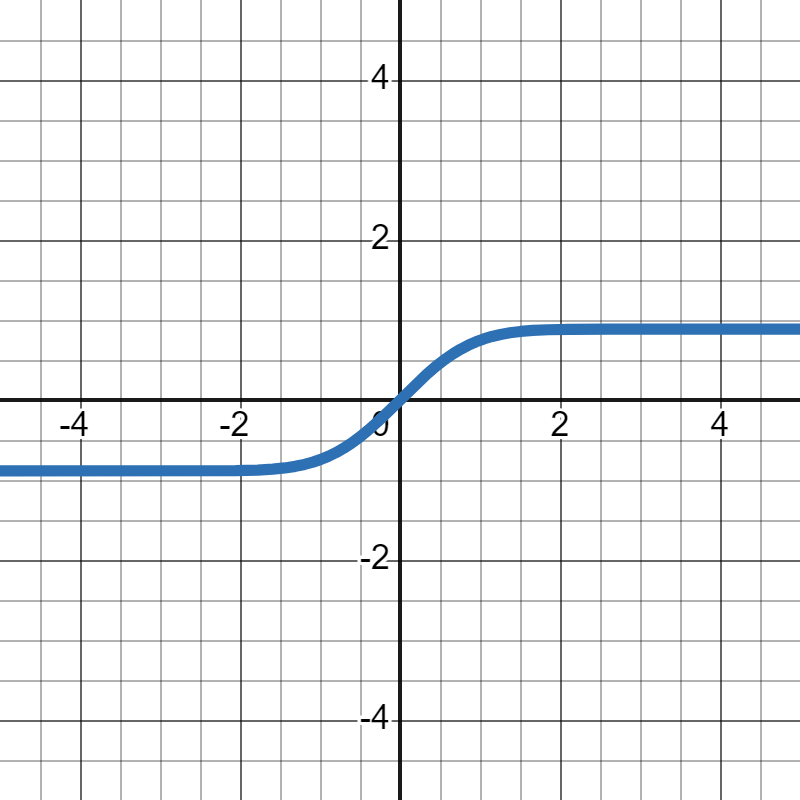
\includegraphics[width=1\textwidth]{err}}%
  \caption{График функции ошибок $\Phi(z) = \int\limits_0^{z} e^{-x^2}dx$}
  \label{fig:err_int}
  \end{figure}%
\end{minipage}\hspace{10pt}%
\begin{minipage}[t]{.4\textwidth}%
\begin{figure}[H]
  \centering
  \fbox{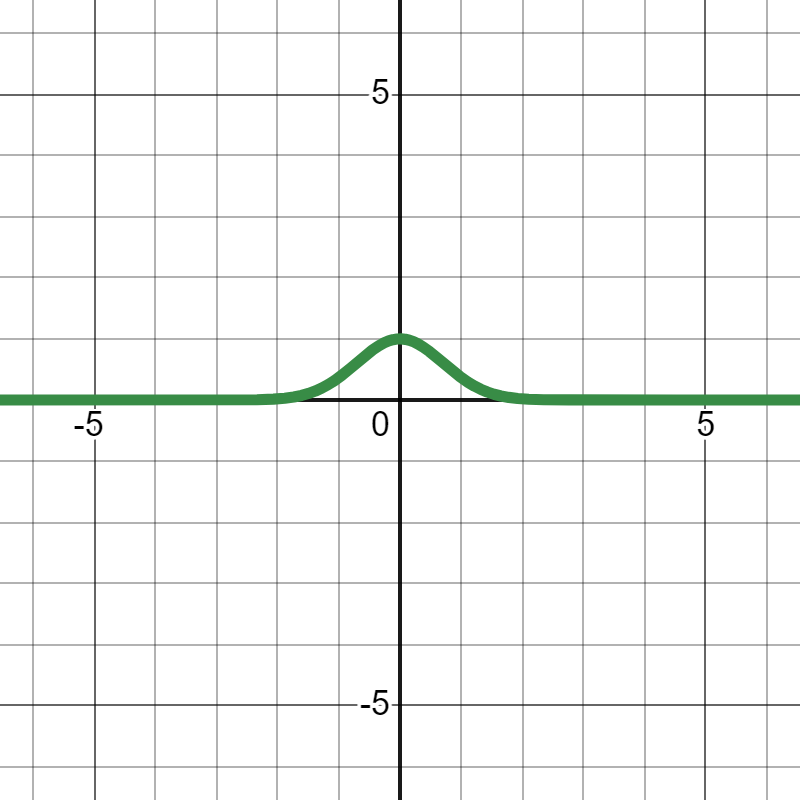
\includegraphics[width=1\textwidth]{err_fun}}%
  \caption{График подынтегральной фукнции для функции ошибок $y =  e^{-x^2}$}
  \label{fig:err_fun}
    \end{figure}
\end{minipage}
\end{figure}

\begin{figure}[H]
\centering
\begin{minipage}[t]{.4\textwidth}
\begin{figure}[H]
  \centering
  \fbox{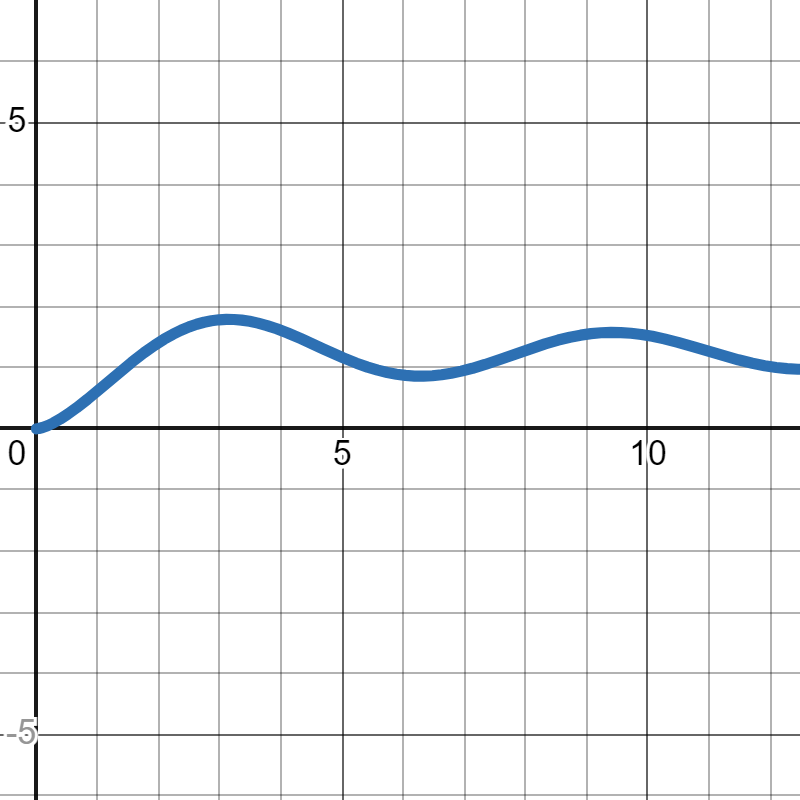
\includegraphics[width=1\textwidth]{fren1}}%
  \caption{График интеграла Френеля $\Phi_{S}(z) = \int\limits_0^{z} \frac{\sin{t}}{\sqrt{t}} dt$}
  \label{fig:fren1_int}
  \end{figure}%
\end{minipage}\hspace{10pt}%
\begin{minipage}[t]{.4\textwidth}%
\begin{figure}[H]
  \centering
  \fbox{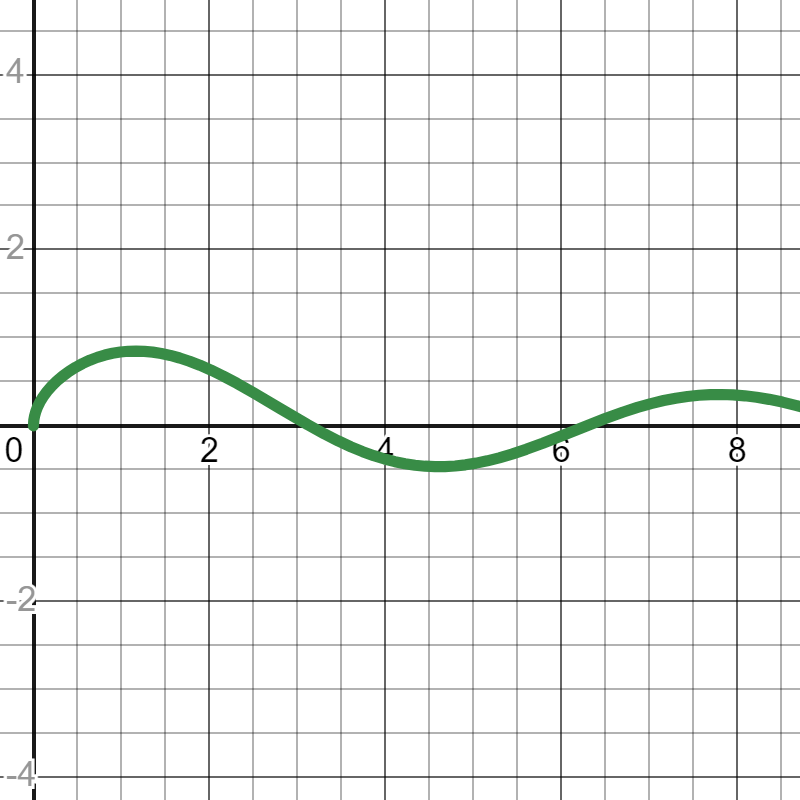
\includegraphics[width=1\textwidth]{fren1_fun}}%
  \caption{График подынтегральной функции для фукнции Френеля $y =  \frac{\sin{x}}{\sqrt{x}}$}
  \label{fig:fren1_fun}
    \end{figure}
\end{minipage}
\end{figure}

\begin{figure}[H]
\centering
\begin{minipage}[t]{.4\textwidth}
\begin{figure}[H]
  \centering
  \fbox{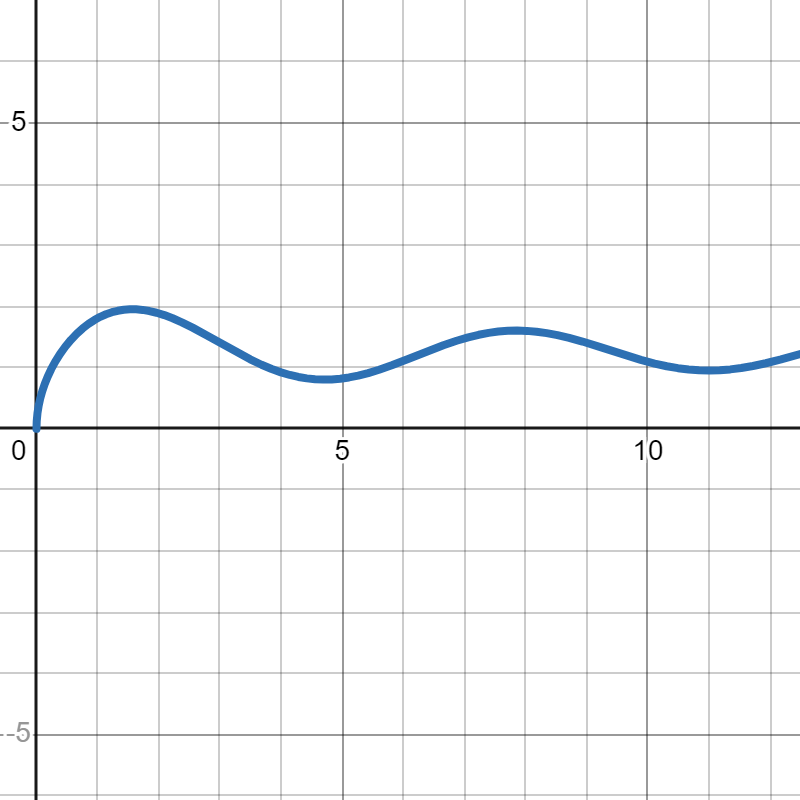
\includegraphics[width=1\textwidth]{fren2}}%
  \caption{График интеграла Френеля $\Phi_{S}(z) = \int\limits_0^{z} \frac{\cos{t}}{\sqrt{t}} dt$}
  \label{fig:fren2_int}
  \end{figure}%
\end{minipage}\hspace{10pt}%
\begin{minipage}[t]{.4\textwidth}%
\begin{figure}[H]
  \centering
  \fbox{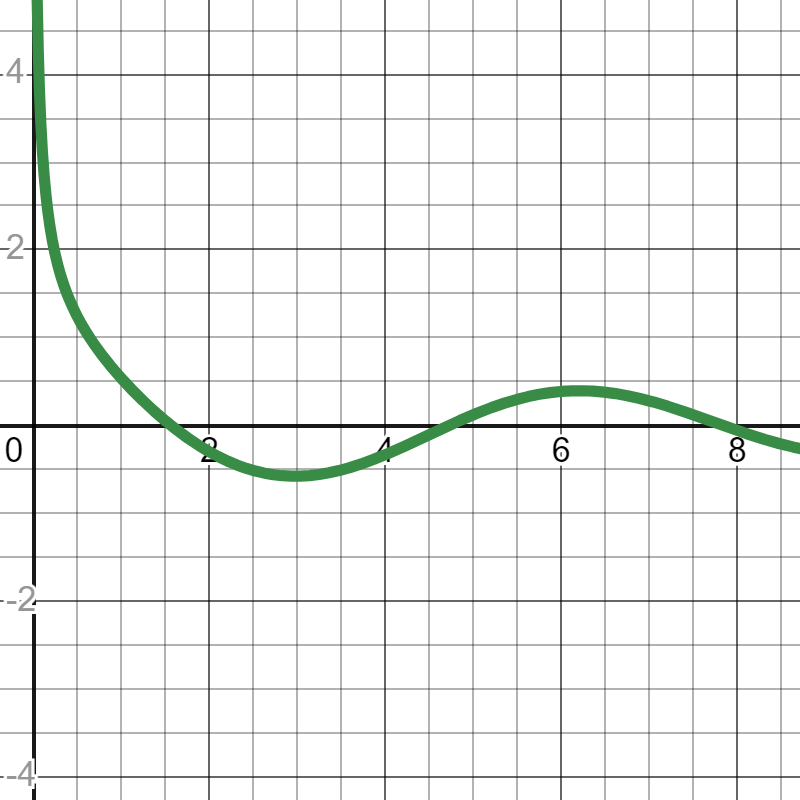
\includegraphics[width=1\textwidth]{fren2_fun}}%
  \caption{График подынтегральной функции для фукнции Френеля $y =  \frac{\cos{x}}{\sqrt{x}}$}
  \label{fig:fren2_fun}
    \end{figure}
\end{minipage}
\end{figure}


\end{document}



